\chapter{The transmission of the Welsh laws}
\label{cha:welsh-laws}

In this chapter, I analyze where lenition was represented in the various law texts, which have existed in a written form since at least the early thirteenth century and which continued to be copied throughout the remainder of the \gls{mw} period. Taken together, these factors indicate that the law texts lend themselves to investigation of the methods  scribes used to copy manuscripts and under what circumstances they maintained or changed the non-representation of lenited voiceless stops.

Lenition of voiceless stops was represented orthographically by the mid-fourteenth century, so manuscripts from around this period are most useful to chart this change in orthography.
Earlier manuscripts  demonstrate that the law texts did see a period in which lenition of voiceless stops was not represented, even though lenition of other consonants was.
Later manuscripts may still show traces of the early orthography, allowing identification of specific environments within which non-representation of lenited voiceless stops may be preserved.
I focus on the transmission of \mw{Llyfr Iorwerth}, because this text can be found in most of the oldest law manuscripts as well as some of the newer ones. Earlier research indicates that none of the surviving manuscripts may be considered the original composition:
\tqt{{[N]}o MS.\ of those now extant can be regarded as the original Book of Iorwerth, for none of them is such that the others may reasonably be held to be derived from it. Nevertheless, it is probable that all of the Venedotian MSS.\ were copied directly or indirectly from a common archetype of the class, for there is too much similarity between them to allow a belief in their independent origin.}{wiliam_llyfr_1960}{xxi}
The fact that all extant manuscripts go back to one single written source well before orthographical lenition of voiceless stops means that we may safely assume that all instances of orthographically lenited voiceless stops found in these manuscripts are the result of scribal innovation arising from copying this text. 

% How are various manuscripts related to each other?
% It is nowadays thought that none of the earliest extant manuscripts is a direct ancestor of another extant copy.
% One author who did think this was J.\ Gwenogvryn Evans (Figure~\ref{fig:gwevanslli}).
% Rather, extant manuscripts are held to have common exemplars that no longer exist.
% Figure~\ref{fig:stemmatestb} gives a stemma for the Iorwerth manuscripts (and some more manuscripts), and I will use this stemma as a point of departure for my own research.

% Which manuscripts may be used for analysis?
% One useful manuscript is \textit{A}, the \gls{bbch}, dating from around 1250. This manuscript is one of the oldest law manuscripts, and its orthography is very unusual.
% Another useful manuscript is \textit{B}, which is also fairly old, and dates from the end of the thirteenth century.
% Other thirteenth-century manuscripts shown in Figure~\ref{fig:stemmatestb}: \textit{EC};
% early fourteenth century: \textit{G};
% other manuscripts in this stemma are all later than the fourteenth century.
% Some more useful manuscripts are: \textit{VW}, by scribe X86; \textit{Tr}, by Gwilym Was Da.

% What sections of the law texts are useful for analysis?
% Figure~\ref{fig:stemmatestb} shows that \textit{B} was  transmitted in part from several sources. This makes both the Test Book and the Laws of Country interesting targets for analysis, as the orthography of lenition may confirm or deny this peculiar reconstruction by Charles-Edwards.
% Figure~\ref{fig:stemmatestb} also shows that different parts of the Test Book may have been added in intermediate stages between Redaction I and the extant manuscripts.
% Comparison of these chunks with text found in all the manuscripts may prove useful in establishing at what point in time these chunks were added, and therefore when some of the hypothetical nodes in the stemma were written.

% \subsection{The law corpus}
% \label{sec:fleshed-out-research}
I analyse a part of the tractate on suretyship, which is found in many manuscripts from the Iorwerth tradition, and those manuscripts vary in date from the mid-thirteenth century to 1404.
To be more specific, I use \textcite[\S\S58--65]{wiliam_llyfr_1960} for analysis. The tractate of suretyship is particularly suitable for analysis because it constitutes an archaic core of the Iorwerth law tradition and may, therefore, safely be assumed to have had a textual form well before the dates of the first manuscripts which date from the mid-thirteenth century\footnote{Compare, for instance \S101 on suretyship, on which \textcite[20]{stacey_archaic_1986} describes the Iorwerth version as preserving the most primitive version.}. We may consequently be fairly certain that lenition of voiceless stops was not represented orthographically in the latest shared ancestor of all the extant manuscripts.

\section{On the manuscripts}
\label{sec:manuscripts}
This section discusses the eight manuscripts used for analysis, which are referred to by their manuscript sigla throughout the chapter. These manuscript sigla were coined by \textcite{owen_ancient_1841}.
The manuscript with the siglum \gls{sA} is  \gls{nlw}, Peniarth MS 29, also known as the Black Book of Chirk, dated to the mid-thirteenth century, and thought to have been produced in the Arfon region~\autocite[171]{Rus_Scribal95}.
Several scribes may be identified in the manuscript, but the material used here comes from Hand D and a few lines by Hand E~\autocite[133--134]{Rus_Scribal95}.
Hand D's orthography is peculiar for the thirteenth century in that he writes /ə/ with \mw[]{a}, and he has many variant spellings for /θ/, such as \mw[]{s, h, sh, ht, sth}.
Hand E's work seems to be `the most regular and consistent of all scribes in [\gls{sA}]'~\autocite[152]{Rus_Scribal95}.
The irregular spelling of dental fricatives, along with some other orthographical irregularities, suggests that \gls{sA}'s exemplar was written in \gls{ow} orthography~\autocite[169]{Rus_Scribal95}. 

Manuscript \gls{sB} is also known as \acrshort{bl}, Cotton Titus MS D.~ii, which belongs to the late thirteenth century and may have been produced in St Asaph~\autocite[v]{elias_golygiad_2007}. The orthography of \gls{sB} is more consistent than that of \gls{sA}. \Textcite[xlii]{wiliam_llyfr_1960} notes about the orthography that `[m]utations of initial consonants are sometimes indicated, sometimes not. The nasal mutation, however, is regularly shown'.

Manuscript \gls{sC} is known  as \gls{bl}, Cotton Caligula MS A.~iii, and may be dated to the mid-thirteenth century. Its scribe was the same scribe as the one of the \gls{ll1} and \gls{p44} manuscripts discussed in Chapter~\ref{cha:indep-comp-mwbr}. \Textcite[189]{huws_medieval_2000} argues that the manuscript was probably written in a monastic milieu in north-east Wales. He considers Valle Crucis in Denbighshire to be the most likely place of composition.

Manuscript \gls{sD} is also known as \gls{nlw}, Peniarth MS 32, and as \mow[]{Y Llyfr Teg}. It was produced around 1404~\autocite[60]{huws_medieval_2000} in the Cwm Tawe area~\autocite[v]{elias_golygiad_2007}. The laws texts are all written by Scribe X91, who is described as writing with great regularity and legibility and with orthography mostly conforming to what was expected in this period~\autocite{thomas_tei_2013}.

Manuscript \gls{sE} is more fully known as \gls{bl} Additional MS 14931,  produced at the end of the thirteenth century, and  considered a sister manuscript to \gls{sA}. An addition was written near the end in the hand of \gls{sB}. This identification with \gls{sA} and \gls{sB} imply a geographic connection either to Arfon or to St Asaph~\autocite[100]{charles-edwards_welsh_1989}.

Manuscript \gls{sG} is \gls{nlw}, Peniarth MS 35, written in the early fourteenth century by a scribe  Daniel Huws identifies as X87, who also copied the laws of the Cyfnerth group from south Wales~\autocite{smith_tei_2013}. \Gls{sG} was probably produced in the Brycheiniog area~\autocite[v]{elias_golygiad_2007}. It is the first manuscript from the Iorwerth tradition with a southern provenance~\autocite{charles-edwards_introduction_1986}.

Manuscript \gls{sJ} is Oxford, Jesus College MS 57, and was written around 1400 by Hywel Vychan of Builth, who was also the principal scribe of the Red Book of Hergest~\autocite[100]{charles-edwards_welsh_1989}. The manuscript may be connected to the Cwm Tawe area~\autocite{james_llwyr_1993}.

Manuscript \gls{sK} is also known as \gls{nlw}, Peniarth MS 40, or as \mw{Llyfr Calan}, and is written after 1469 by Lewis Glyn Cothi~\autocite{roberts_cyfraith_2011}. It contains four poems in the beginning addressed to the lord of Cefn Llys, suggesting that the manuscript was written in this area~\autocite[374]{evans_report_1899}.

The paragraphs selected for analysis correspond to the folio numbers, column numbers, and line numbers in the manuscripts given in Table~\ref{tab:surety}. This text runs continuously in all of these manuscripts, except in \gls{sG}, where it is interspersed with other additions. Over 200 data points were taken from each manuscript for analysis, except for \gls{sJ}, which has shortened the tractate on suretyship considerably.  
\begin{table}[h]
  \centering
 \begin{tabular}{lddlld}
  \toprule
  MS            & Begin                   & End   & Date & Location                   & Data pts     \\ \midrule
  \gls{sA}            & 43.22                   & 48.11  & s.xiii\textsuperscript{med}             & Arfon  & 210         \\
  \gls{sB}            & 20r.22                  & 23v.17 & s.xiii\textsuperscript{2}      & St Asaph  & 234         \\
  \gls{sC}            & 155va.10                 & 161ra.7 & s.xiii\textsuperscript{med}              & Valle Crucis  & 229         \\
  \gls{sD}            & 52.19                   & 61.16  & ca.\ 1404         & Cwm Tawe  & 231         \\
  \gls{sE}            & 34.5                   & 39.13  & s.xiii\textsuperscript{2}     & Arfon/St Asaph   & 218         \\
  \multirow{2}{*}{\gls{sG}}   & 20r.1                   & 23v.11  & \multirow{2}{*}{s.xiv\textsuperscript{1}}& \multirow{2}{*}{Brycheiniog}  & \multirow{2}{*}{263} \\
                & 26r.1                   & 26v.12 &                     &  &           \\
   \gls{sJ} & 269.19 & 277.11 & ca.\ 1400 & Cwm Tawe & 147 \\
  \gls{sK}&68.19 & 77.23 & s.xv\textsuperscript{2}& Cefn Llys & 244 \\
  \bottomrule
 \end{tabular}
 \caption{Location of  \mw{Llyfr Iorwerth} §§~58–65, per manuscript.}
  \label{tab:surety}
\end{table}

\subsection{The geographical spread of the manuscripts}
\label{sec:geogr-spre-manuscr}

Figure~\ref{fig:mslocs} illustrates the places where the manuscripts are presumed to have been produced. The geographic origin of a manuscript tends to be less certain than its date, which means that the locations on the map may be taken with a grain of salt. Still, it is reasonable that these localisations are not off by an order of magnitude, and that we may somewhat confidently classify the manuscripts geographically into two groups a northern group and a southern group. The first  comprises \gls{sA}\gls{sB}\gls{sC}\gls{sE}; all of these manuscripts may be dated to the thirteenth century. The second group  comprises \gls{sD}\gls{sG}\gls{sJ}\gls{sK}; all of these manuscripts are from the fourteenth and fifteenth century.

\begin{figure}[h]
  \centering
  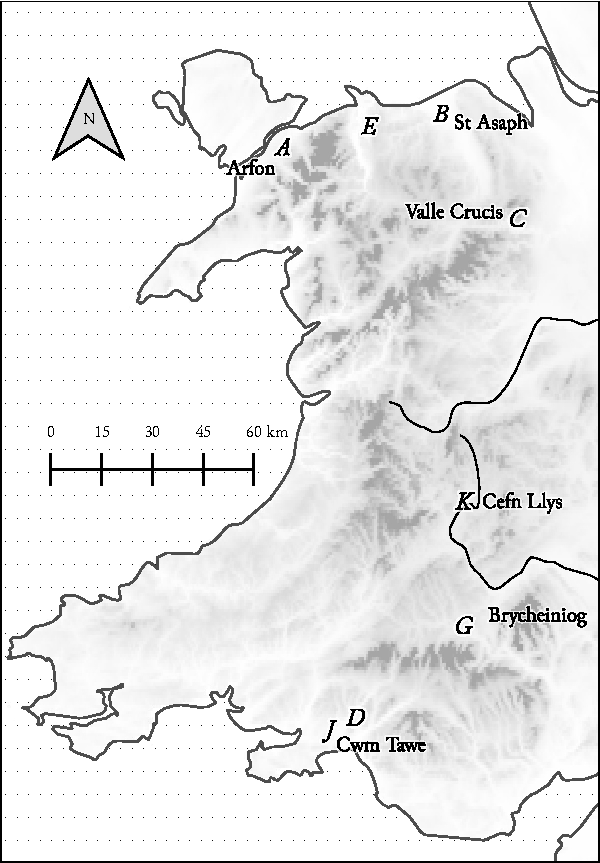
\includegraphics{3orth/images/mslocations.pdf}
  \caption[Locations of the law manuscripts.]{Locations of the law manuscripts analysed in this chapter. \gls{sE} is plausibly connected to both Arfon and St Asaph, so it stands halfway between them.}
  \label{fig:mslocs}
\end{figure}

Because the geographical split and temporal split occur along the same lines, it is difficult to separate whether the different patterns of lenition found in these manuscripts are caused by their temporal distance or their geographical distance.

\section{The stemmatic relationship of the manuscripts}
\label{sec:stemmata}
No manuscript named here has a surviving exemplar and all manuscripts share a common written ancestor. Despite the lack of surviving exemplars to the manuscripts discussed in this chapter, a rough stemmatic relationship between the manuscripts has been uncovered through text-critical methods. Figure~\ref{fig:twostemmata} shows two of the most recent insights into their derivation from a common ancestor, and the manuscripts that may be considered to form independent subgroupings.

\begin{figure}[h]
  \newlength{\stemmalen}
  \setlength{\stemmalen}{2.5cm}
  \begin{subfigure}[b]{0.5\linewidth}
    \centering
    \begin{forest} for tree={font=\itshape,l=10mm,l sep=0mm,s sep=3mm,delay={where content={}{shape=coordinate}{}}}
      [X
      [α
      [γ
      [\gls{sA},l=20mm]
      [\gls{sE},l=25mm]
      ]
      [\gls{sC},l=30mm]
      ]
      [β
      [δ
      [\gls{sD},l=5.3cm,s=-6mm]]
      [ε
      [\gls{sG},l=35mm,s=-6mm]
      [ζ,s=6mm
      [\gls{sB},l=15mm]
      [\gls{sJ},l=4.3cm]
      [\gls{sK},l=5.5cm,s=6mm]
      ]
      ]
      ]
      ]
      \node at (forest cs:l=3cm,s=\stemmalen +.5cm) {1200};
      \node at (forest cs:l=5cm,s=\stemmalen +.5cm) {1300};
      \node at (forest cs:l=7cm,s=\stemmalen +.5cm) {1400};
      \node at (forest cs:l=9cm,s=\stemmalen +.5cm) {1500};
      \draw[dotted] (forest cs:l=3cm, s=-\stemmalen) -- (forest cs:l=3cm, s=\stemmalen);
      \draw[dotted] (forest cs:l=5cm, s=-\stemmalen) -- (forest cs:l=5cm, s=\stemmalen);
      \draw[dotted] (forest cs:l=7cm, s=-\stemmalen) -- (forest cs:l=7cm, s=\stemmalen);  
      \draw[dotted] (forest cs:l=9cm, s=-\stemmalen) -- (forest cs:l=9cm, s=\stemmalen);  
    \end{forest}
    \caption{\textcite[138]{charles-edwards_iorwerth_1986}}
  \end{subfigure}%
  \begin{subfigure}[b]{0.5\linewidth}
    \centering
    \begin{forest} for tree={font=\itshape,l=10mm,l sep=0mm,s sep=3mm,delay={where content={}{shape=coordinate}{}}}
      [\textup{Redaction I}
      [α
      [\gls{sA},l=30mm]
      [\gls{sE},l=35mm]
      ]
      [\textup{Redaction II}
      [β
      [\gls{sC},l=20mm]
      ]
      [γ,
      [
      [\gls{sD},s=-6mm,l=4.3cm]
      [\gls{sG},l=25mm]]
      [
      [\gls{sB},s=0mm,l=15mm]
      [\gls{sJ},l=4.3cm,s=0mm]
      [\gls{sK},l=55mm,s=6mm]
      ]
      ]
      ]
      ]
      ]
      \node at (forest cs:l=3cm,s=\stemmalen +.5cm) {1200};
      \node at (forest cs:l=5cm,s=\stemmalen +.5cm) {1300};
      \node at (forest cs:l=7cm,s=\stemmalen +.5cm) {1400};
      \node at (forest cs:l=9cm,s=\stemmalen +.5cm) {1500};
      \draw[dotted] (forest cs:l=3cm, s=-\stemmalen) -- (forest cs:l=3cm, s=\stemmalen);
      \draw[dotted] (forest cs:l=5cm, s=-\stemmalen) -- (forest cs:l=5cm, s=\stemmalen);
      \draw[dotted] (forest cs:l=7cm, s=-\stemmalen) -- (forest cs:l=7cm, s=\stemmalen);  
      \draw[dotted] (forest cs:l=9cm, s=-\stemmalen) -- (forest cs:l=9cm, s=\stemmalen);  
    \end{forest}
    \caption{\textcite{charles-edwards_textual_2016}}
  \end{subfigure}
  \caption{Two stemmata of the tractate on suretyship.}
  \label{fig:twostemmata}
\end{figure}

Both stemmata in Figure~\ref{fig:twostemmata} give a similar account of how the law manuscriopts are related. They differ in two aspects. Both stemmata show a particularly close relationship between \gls{sA}\gls{sE} on one hand and \gls{sB}\gls{sD}\gls{sG}\gls{sJ}\gls{sK} on the other hand. They disagree on which of these two groups \gls{sC} is the closest to. The other point they disagree on is the position of \gls{sG}, which may either be closer to \gls{sB}\gls{sJ}\gls{sK} or to \gls{sD}.
  
% \section{Some preliminary observations}
% \label{sec:some-prel-observ}

% \gls{sB}, folio 42v, §~104 has the following as the preface of the Test Book:
% \mwcc[preftestb]{\gls{sB} 42v.18--20}{Llyma e dechreu e Llyuer Prauf. Sef yu henne, teyr colouen keureyth guerth guyllt a dof ac a perthyn arnadunt.}{Here starts the Test Book. That is, three columns of law of wild and tame value, and what relates to them.}
% \todo[inline]{refer to lawyers and laymen: test book is later addition, not found in AC(?), dates node in stemma}
% This one excerpt shown in Example~\ref{preftestb} shows lenition word-internally, but it contains two instances where word-initial lenition may be expected, but is not found: \mw[columns of law]{colouen keureyth}, with lenition following a feminine noun, and \mw[that relates]{a perthyn}, with lenition following the verbal particle.
% As lenition  is not written here, we may assume that Redaction II was composed before lenition of voiceless stops was written.
% This is unsurprising, as one of its manuscripts, \gls{sC}, itself  as early as 1250.
% This somewhat trivial example serves to demonstrate how combined knowledge of when which parts were added in a stemma and of the orthography of lenition may help to date hypothetical nodes in a stemma. 

\section{How manuscripts modernize}
\label{sec:how-do-manuscripts}

How is lenition modernized in the later manuscripts compared to the older ones?
The most obvious way of course is by simply writing lenition where no lenition was written previously. Such innovations are easily covered by simply verifying the extent to which each manuscript represents lenition where it is expected from the grammar. However, older orthographies may also be modernised in more insidious ways.

When older manuscripts have an element that causes lenition followed by a word starting with a voiceless stop, lenition is typically not written. Later recensions sometimes solve this outdated orthographical convention by simply deleting the element causing lenition, as demonstrated by comparisons of \gls{sD} found in Examples~\ref{ex:ekyfreithd} and \ref{ex:ykeinhawcd} with its  older cousin \gls{sB} found in Examples~\ref{ex:ekyfreithb} \ref{ex:ykeinhawcb}:
\begin{mwl}
  \mwc[ex:ekyfreithb]{\gls{sB} 20v.24}{sef a wyl \al{e keureyth} ena}{This is how the law sees it}
  \mwc[ex:ekyfreithd]{\gls{sD} 54.3}{Sef a wyl \al{kyfreith} yna}{This is how [the] law sees it}
  \mwc[ex:ekyfreithk]{\gls{sK} 70.6}{Sef a ỽyl .k.\ yna}{This is how [the] law sees it}
  \mwc[ex:ykeinhawcb]{\gls{sB} 21v.22--24}{ny dyweyt \al{e keureyth} deleu ohanau trae keuen namen dymey canys dymey yu traean \al{e keynnyauc} keureyth.}{The  law does not say that he is  entitled, except to a halfpenny back, because that is a third of the penny of law.}
  \mwc[ex:ykeinhawcd]{\gls{sD} 56.19--21}{Ny dyweit.\ \al{k\abbr{yfreith}.}\ dylyu ohonaỽ drachefyn namyn dimei. kanys hynny yỽ traean \al{keinhaỽc} k\abbr{yfreith}.}{{[}The] law does not say that he is  entitled, except to a halfpenny back, because that is a third of [the] penny of law.}
\end{mwl}
The more archaic wording in \gls{sB} is shared with most other manuscripts, but Example~\ref{ex:ekyfreithk} shows that the scribe of \gls{sK} also applied this strategy of deletion. The lack of definite articles in \gls{sD}  makes for awkward sentences in both cases. These awkward sentences are evidence that \gls{sD} had an exemplar that  lacked orthographical lenition following the article, because this wording without the definite article would not be expected if \gls{sD} contained a contemporary fifteenth-century text. Another instance that shows removal of the element that causes lenition is  Example~\ref{ex:unceiniogd}, where \gls{sD} preserves an original leniting \mw[one]{un}. In this case, it is \gls{sK} in Example~\ref{ex:unceiniogk} which innovates in this manner. These examples show that this rewording is a haphazard and inconsistently applied tactic, even though the scribe of \gls{sD} is otherwise quite prolific in rewording. It also shows that this tactic is not unique to \gls{sD}.
\begin{mwl}
    \mwc[ex:unceiniogd]{\gls{sD} 56.16--18}{O chanhatta y kynnogyn yr mach rodi gỽystyl punt yn ỻe \al{un geinyaỽc}}{If the debtor allows the surety to give a pound's pledge instead of one penny}
  \mwc[ex:unceiniogk]{\gls{sK} 72.22--23}{O chanhiatta y kynogyn ir mach rodi gỽystyl punt yn lle \al{k\abbr{einiawc}}.}{If the debtor allows the surety to give a pound's pledge instead of one penny}
\end{mwl}
Existential verb \mw[]{oes} causes lenition, as is shown by Example~\ref{ex:ardelwkynogynd}. Example~\ref{ex:ardelwkynogynk} shows that words may not only be removed, but also added in order to make a lack of lenition grammatical: the scribe of \gls{sK} inserted \mw[]{ardelw} in order to make sense of non-lenited \mw{kynogyn} following \mw[]{oes}.
\begin{mwl}
  \mwc[ex:ardelwkynogynd]{\gls{sD} 58.4}{OS o uechni y dewis; nyt oes \al{gynnogyn}.}{If he chooses [his legal role] as a surety, there is no debtor.}
  \mwc[ex:ardelwkynogynk]{\gls{sK} 74.15--16}{Os o uechni i deỽis i ardelỽ.\ it oes \al{ardelỽ kynogyn}.}{If he chooses his legal role as a surety, there is no legal role of a debtor.}
\end{mwl}
The way these scribes updated an older orthographical stratum by  deleting the environments causing lenition is particularly insidious, because it does not show up in the statistics. After all, no instance of non-represented lenition exists if the environment is reworked so as not to require lenition in the first place. However, these examples demonstrate that if we see an odd-looking non-leniting element or we see an odd-looking absence of a leniting element in a post-1300 manuscript, then this may be indicative of an older orthographical stratum. In practice, however, this knowledge may be hard to apply in establishing that an old text in a new manuscript is indeed old. Comparing \gls{sD} with its cousins demonstrates how its scribe modernized by removing the article, but it the change is only obvious after comparing this manuscript with  its cousins in the first place. It remains to be seen whether it would be possible to diagnose the removal of a feminine article or some other element causing lenition in a late \gls{mw} manuscript and then conclude that it had an early exemplar, without any thirteenth-century manuscript to compare it with. It would be highly trivial to demonstrate a text has a thirteenth-century orthographical stratum, if one can only do so by comparing it with a different manuscript indeed found in the thirteenth century.
\section{Results}
\label{sec:results}

Table~\ref{tab:lenlawcountryboth} shows to what degree lenition was represented in the tractate on suretyship in various recensions of the book of Iorwerth. One obvious difference between the results shown in this table and what we see in the results  of Chapter~\ref{cha:indep-comp-mwbr} found in Table~\ref{tab:perlenbrutboth} is that even in the latest recensions fullly consistent representation of  lenition of \mw{p, t, c} is not achieved. The latest manuscript, \gls{sD} written about 1404, still only writes lenition where it should in about three-quarters of the cases. This lack of thoroughness is visualised in Figure~\ref{fig:barchartlaws}.

\begin{table}[h]
  \begin{subtable}[b]{\linewidth}
    \centering
    \begin{tabular}{lddddddd}
      \toprule
      \tch{MS} & \tch{\mw{b}} & \tch{\mw{g}} & \tch{\mw{ll}} & \tch{\mw{m}} & \tch{\mw{p}} & \tch{\mw{t}} & \tch{\mw{c}} \\
      \midrule
      \gls{sA} & 56.0 & 23.1 & 91.7 & 98.0 & 8.3 & 0.0 & 13.0 \\
      \gls{sB} & 72.7 & 95.8 & 100.0 & 96.2 & 64.3 & 0.0 & 46.3 \\
      \gls{sC} & 71.4 & 51.2 & 100.0 & 98.2 & 21.4 & 0.0 & 21.9 \\
      \gls{sD} & 68.0 & 97.8 & 100.0 & 94.7 & 83.3 & 76.5 & 88.7 \\
      \gls{sE} & 71.4 & 100.0 & 83.3 & 96.2 & 96.2 & 58.8 & 92.9 \\
      \gls{sG} & 76.9 & 100.0 & 100.0 & 98.3 & 46.9 & 41.2 & 59.3 \\
      \gls{sJ} & 90.9 & 100.0 & 100.0 & 93.9 & 90.5 & 80.0 & 91.2 \\
      \gls{sK} & 80.0 & 98.2 & 100.0 & 96.2 & 51.6 & 18.8 & 71.0 \\
      \bottomrule
    \end{tabular}%
    \caption{Including research exceptions.}
    \label{tab:lenlawcountryincre}%
  \end{subtable}
  \begin{subtable}[b]{\linewidth}
    \centering
    \begin{tabular}{lddddddd}
      \toprule
      \tch{MS} & \tch{\mw{b}} & \tch{\mw{g}} & \tch{\mw{ll}} & \tch{\mw{m}} & \tch{\mw{p}} & \tch{\mw{t}} & \tch{\mw{c}} \\
      \midrule
      \gls{sA} & 56.0 & 23.1 & 91.7 & 97.9 & 10.5 & 0.0 & 10.0 \\
      \gls{sB} & 72.7 & 95.8 & 100.0 & 95.8 & 52.4 & 0.0 & 12.2 \\
      \gls{sC} & 71.4 & 51.2 & 100.0 & 98.0 & 0.0 & 0.0 & 0.0 \\
      \gls{sD} & 68.0 & 97.8 & 100.0 & 93.9 & 79.2 & 73.3 & 78.6 \\
      \gls{sE} & 71.4 & 100.0 & 83.3 & 95.7 & 95.2 & 46.2 & 88.6 \\
      \gls{sG} & 76.9 & 100.0 & 100.0 & 98.0 & 32.0 & 35.5 & 29.4 \\
      \gls{sJ} & 90.9 & 100.0 & 100.0 & 93.5 & 88.2 & 76.9 & 83.3 \\
      \gls{sK} & 80.0 & 98.2 & 100.0 & 95.3 & 34.8 & 13.3 & 55.0 \\
      \bottomrule
    \end{tabular}%
    \caption{Excluding research exceptions.}
    \label{tab:lenlawcountryexcre}%
  \end{subtable}
  \caption{Representation of lenition in various recensions of the tractate on suretyship.}
  \label{tab:lenlawcountryboth}
\end{table}%


Another difference is found specifically by comparing the numbers between both parts of Table~\ref{tab:lenlawcountryincre}, and concerns research exceptions, \ie instances where lenition is not synchronically morphophonemic, such as \mw[with]{gan}, or \mw[\mbox{-ever}]{bynnac}. The orthography of lenition in these exceptions only differs from \gls{morphophonlen} when the initial consonant is a voiceless stop, indicating that degrammaticalized lenition of voiceless stops was written early on, but not grammatical lenition. The greatest differences between these percentages is found in \gls{sB}, because this manuscript both fails to write morphophonemic lenition and starts writing words like \mw[with]{gan} with a lenited grapheme. In \gls{sA}, and to a lesser degree \gls{sC}, lenition is regularly not written even when dealing with \gls{petr}, while the other manuscripts begin to modernise the orthography of grammatical lenition and show lenition in these instances.

\Gls{sA} and \gls{sC} do not represent lenition of \mw{g} consistently. The former hardly ever does so, while the latter does so in about half the cases. In \gls{sA}, most instances of orthographical lenition comprise either an inflected form of the verb meaning `to counterswear', \eg \gls{sA} 44.28 \mw{vrhtegho}, or `be able', \eg \gls{sA} 45.34 \mw{eill}. In \gls{sC} we see that words of the type /gw̯\gls{C}/ seldom lenite, as with some translations of the \mw{Brut}\footnote{See Section~\ref{sec:lenited-mwg}}. These observations about both manuscripts fall short of full explanations for the distribution between lenited and unlenited \mw{g}, but they nevertheless offer a valuable insight. The fact that these two orthographically conservative manuscripts both fail to lenite \mw{g} demonstrates that their common ancestor did not write lenition of \mw{g}. This change is obscured by the high degree of success with which other manuscripts modernized the spelling of lenited \mw{g}, and leaves one to wonder why this modernization was done so much more successfully in the case of \mw{g} than in the case of \mw{p, t, c}.

\begin{figure}[h]
  \centering
  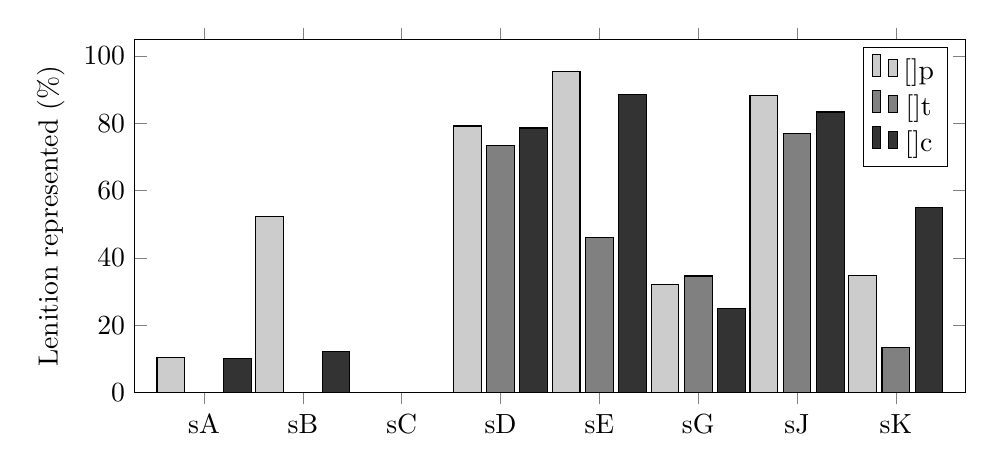
\begin{tikzpicture}
    \begin{axis}[
      ybar,
      ymin=0,
      width=\linewidth,
      height=.5\linewidth,
      % xlabel=Manuscript,
      ylabel={Lenition represented (\%)},
      symbolic x coords={
        \gls{sA},\gls{sB},\gls{sC},\gls{sD},
        \gls{sE},\gls{sG},\gls{sJ},\gls{sK}},
      xtick=data,
      ]
      \addplot [fill=black!20] coordinates {
        (\gls{sA},10.53)
        (\gls{sB},52.38)
        (\gls{sC},0.00)
        (\gls{sD},79.17)
        (\gls{sE},95.24)
        (\gls{sG},32.00)
        (\gls{sJ},88.24)
        (\gls{sK},34.78)
      };
      \addplot [fill=black!50] coordinates{     
        (\gls{sA},0.00)
        (\gls{sB},0.00)
        (\gls{sC},0.00)
        (\gls{sD},73.33)
        (\gls{sE},46.15)
        (\gls{sG},34.62)
        (\gls{sJ},76.92)
        (\gls{sK},13.33)
      };
      \addplot [fill=black!80] coordinates{
        (\gls{sA},10.00)
        (\gls{sB},12.20)
        (\gls{sC},0.00)
        (\gls{sD},78.57)
        (\gls{sE},88.57)
        (\gls{sG},25.00)
        (\gls{sJ},83.33)
        (\gls{sK},55.00)
      };
      \legend{\mw[]{p},\mw[]{t},\mw[]{c}}
    \end{axis}
  \end{tikzpicture}
  \caption{Representation of \lT\ in the tractate on suretyship, excluding research exceptions.}
  \label{fig:barchartlaws}
\end{figure}


No manuscript fully represents lenition of \mw{b} in all cases. However, more than half of these instances involve inflections of \mw[to be]{bot} following the negative particle \mw{ny, na} or compounds containing the same particle: \mw{ony}. This merely sporadic lenition of \mw{bod} following the negative particle is still found in present-day Welsh \autocite[695]{thomas_gramadeg_1996}. Failure to lenite following \mw{ny} is also found with other verbs starting with \mw{b}, and with verbs starting with \mw{m}. Lack of orthographical lenition may mirror lack of phonemic lenition in this specific context, and this pattern is, therefore, irrelevant to the topic of the orthography of lenition. 




\section{Chronology and geography in the results}
\label{sec:chronology-laws}

This section discusses how the percentages given in Table~\ref{tab:lenlawcountryexcre} correspond to the date of composition of the manuscript. One hypothesis is that a law manuscript's orthography is more conservative than that of a contemporary manuscript containing the \mw{Brut}, because the former would  copy the orthography of an older Welsh-language exemplar, and the latter would be a new Welsh composition fully adopting the orthography of its time. Another hypothesis is that lenition is modernised more frequently at later dates than it is shortly after lenited voiceless stops came to be represented, because the habit of representing lenition would become more ingrained over time.

\subsection{The apparent age of \gls{sA} and \gls{sC}}
\label{sec:glsa--glsc}
The earliest two manuscripts are mid-thirteenth-century \gls{sA} and \gls{sC}. As expected, they do not write lenition of voiceless stops, because this orthographical innovation had not taken place yet. These manuscripts show the same pattern as a contemporary original composition would. They date from the same period as \gls{ll1} and \gls{p44} discussed in Chapter~\ref{cha:indep-comp-mwbr}, and indeed show the same pattern of non-lenition of voiceless stops.

Although neither of these manuscripts generally writes lenition of \mw{p, t, c}, a  handful of instances is found in \gls{sA}. These instances are presented in Table~\ref{tab:lenptcsa}.

\begin{table}[h]
  \centering
    \begin{tabular}{ddwql}
    \toprule
    \tch{p.} & \tch{l.} & \tch{Word} & \tch{Translation} & \tch{Reason} \\
    \midrule
    43 & 26 & bieu & owns & [\mw{a}] \\
    45 & 27 & bieu & owns & [\mw{a}]  \\
    46 & 37 & gredu & believe & \mw{e} ‘his' \\
    47 & 22 & genedel & family & \mw{o}  \\
    47 & 24 & g/enedel & family & \mw{o}  \\
    \bottomrule
    \end{tabular}%
\caption{Instances of orthographical lenition of voiceless stops in \gls{sA}.}
  \label{tab:lenptcsa}
\end{table}

Orthographic lenition of \mw[whose … is]{bieu} may be indicative that this verb was petrified here. Lenition here would be due to verbal particle \mw[]{a}, but this particle is not in fact expressed. Also, \mw[]{bieu} is an irregular inflection. Most irregular inflections are forms with \mw[to be]{bod}, so there is grounds for \mw[whose … is]{[a]\gls{l} bieu} to be reanalysed as starting with a radical \mw[]{b} rather than a lenited \mw[]{p}.

\subsection{The apparent age of \gls{sB} and \gls{sE}}
\label{sec:apparent-age-glssb}
The second earliest group of manuscripts consists of late-thirteenth-century \gls{sB} and \gls{sE}. These two manuscripts differ from each other in terms of how frequently lenition is inserted, but have in common that orthographical lenition of \mw[]{t} is less common than the other two voiceless stops.

Among these two manuscripts, the most archaic-looking orthography of lenited voiceless stops is found in \gls{sB}, where \mw{t} is never lenited, and \mw{p} and \mw{c} are lenited sporadically. This distribution is puzzling, as it conforms to no pattern found in Chapter~\ref{cha:indep-comp-mwbr}. There, we witnessed an intermediate period in the development of orthographical lenition of \mw{p, t, c} where \mw{p, t} were not lenited, but where \mw{c} was. This intermediate period is represented by \gls{bd}, which is roughly contemporaneous to \gls{sB} and \gls{sE}. Table~\ref{tab:lenpsbexre} shows that there is no obvious pattern, and a word such as \mw[thing]{peth} is found both lenited and unlenited in the same grammatical contexts.

\begin{table}[h]
  \centering
  \begin{tabular}{ddwql}
    \toprule
    \tch{f.} & \tch{l.} & \tch{Word} & \tch{Translation} & \tch{Reason} \\
    \midrule
    20r & 23 & beth & thing & \mw{ar} \\
    20r & 26 & pleyt & party & \mw{due} \\
    20r & 26 & byeu & owns & [\mw{a}] \\
    20r & 27 & pleyt & party & \mw{due} \\
    20v & 26 & parth & part & \mw{o} \\
    21r & 24 & pleyt & party & \mw{due} \\
    21r & 26 & beth & thing & \mw{ar} \\
    21r & 29 & beth & thing & \mw{ar} \\
    21r & 29 & beth & thing & \mw{ar} \\
    21v & 1 & beth & thing & \mw{ar} \\
    21v & 10 & peth & thing & \mw{ar} \\
    22r & 16 & beth & thing & \mw{am} \\
    22v & 17 & pen & above & prep.\ adj. \\
    23r & 2 & beth & thing & \mw{ar} \\
    23r & 16 & brynno & may buy & \mw{pan} \\
    23r & 18 & perchen & own & \mw{gan} \\
    23r & 23 & peth & thing & \mw{ar} \\
    23r & 25 & perchennauc & owner & \mw{o} \\
    23r & 29 & beth & thing & prep.\ adj. \\
    23v & 1 & beth & thing & prep.\ adj. \\
    23v & 15 & peth & thing & \mw{ar} \\
    \bottomrule
  \end{tabular}%
  \caption{Lenition of \mw{p} in \gls{sB}, excluding research exceptions.}
  \label{tab:lenpsbexre}%
\end{table}%

So what we have is that the scribe of \gls{sB} to add orthographical lenition of \mw{p}, but only in half the cases, and not for \mw{c, t}. \Gls{sB} dates from the second half of the thirteenth century, when orthographical lenition of \mw{c} became commonplace, but not yet \mw{p, t}. These patterns do not fit together easily, but the common denominator here is that lenition of \mw[]{t} was not expressed, while \mw[]{c} was, and \mw[]{p} behaved inconsistently. 

Manuscript \gls{sE} has percentually more lenition represented for \mw[]{p, c} than any other manuscript before the fifteenth century. Apparently, the scribe of \gls{sE} had a much more innovative orthography than the one of \gls{sB}. Still, this describes but does not explain the wildly differing rates of orthographical lenition between \gls{sB} and \gls{sE}.

In \gls{sE}, lenition of \mw[]{p, t, c} is written more frequently than in \gls{sG}, even though \gls{sE} is dated from the latter half of the thirteenth century while \gls{sG} is dated from the beginning of the fourteenth century. The orthography of lenition therefore makes this manuscript look younger. Still, a clue exists as to \gls{sE}'s earlier date: lenition of \mw{c} is written  more frequently than that of \mw{t}. It is typical of late thirteenth-century orthography to write lenition of \mw{c}, sometimes \mw{p}, but typically not \mw{t}. The fact that \mw[]{t} is represented so much less frequently may serve as a clue that \gls{sE} indeed dates to the late thirteenth century.

\subsection{The apparent age of \gls{sG}}
\label{sec:apparent-age-glssg}

This line of reasoning explains why the next oldest manuscript \gls{sG}, had a lower rate of orthographical representation of lenition. By this point, lenition of \mw[]{p, t, c} are represented in roughly equal measure, because the orthographical innovation was complete. 

Different voiceless stops are all represented to a similar degree, but only about a quarter to a third of lenited \mw{p, t, c} are represented as such. This begs the question whether there is any way to account for the distribution of represented and unrepresented lenition. Some regularities may be found. Scribal abbreviations such as the one given in Example~\ref{abbrsg} never show lenition, perhaps because writing lenition here would make abbreviation unrecognizable.
\mwcc[abbrsg]{\gls{sG} 22v.11}{O d\abbr{eruyd}. y wreic rodi bri duỽ ar peth a'e wadu yn \al{k\abbr{yfreith}aỽl}}{If a woman happens to give an oath and to deny it lawfully}
Also, most instances of \mw[his]{y} are followed by orthographical lenition, perhaps in order to disambiguate this pronoun from the article.

Otherwise, lenition is quite haphazardly represented, and the same grammatical context may show orthographical lenition in one instance, but not in the next. No frequently-occurring grammatical context always has lenition, or never has it. This is significant in itself, because it demonstrates that the scribe of \gls{sG} had the ability to insert lenition, but that it had a low priority for him. He would never do so where it could render an abbreviation unintelligible, and he would do so more frequently only where lenition could serve to make meanings clearer.

Manuscript \gls{sE} and \gls{sG} are the only manuscripts discussed that are close to one another in time, but far in distance. Otherwise, the earlier manuscripts tend to be northern and the later ones southern.

Manuscript \gls{sE} dates from the late thirteenth century, and is most likely produced in North Wales, although it defies exact localisation. Manuscript \gls{sG} dates from the early fourteenth century and may be connected to the Brycheiniog area in the Southeast. Based purely on date, it is surprising that \gls{sE} represents lenited \mw[]{p, t, c} so much more frequently than \gls{sG}. The fact that \gls{sE} still represents lenition of voiceless stops at a higher rate than \gls{sG} implies that orthographical lenition was adopted from an earlier date onwards in North Wales than it was in South Wales.

\subsection{The apparent age of \gls{sD} and \gls{sJ}}
\label{sec:apparent-age-glssd}

In \gls{sD} and \gls{sJ}, lenition occurred in equal measure for all consonants. This again implies that orthographical lenition was added well after the end of the thirteenth century. 

The high representation of lenition in \gls{sD} makes it look late, and indeed the manuscript dates from as late as the early fifteenth century. Manuscript \gls{sD} writes lenition of voiceless stops fairly frequently, but more importantly, this frequency is similar for \mw{p}, \mw{t}, and \mw{c}. This is evidence that \gls{sD} may be dated later than manuscripts hitherto discussed.

Remaining instances of non-represented lenition include scribal abbreviations similar to the one found in  Example~\ref{abbrsg}. Table~\ref{tab:lenptcsd} shows all instances of lenition not represented for voiceless stops. It shows that scribal abbreviations account for non-representation of \mw[]{c}, but not for \mw[]{p, t}. The latter look more like the final traces of a general orthography where lenited voiceless stops were not represented.
\begin{table}[h]
  \centering
    \begin{tabular}{ddwql}
    \toprule
    \tch{p.} & \tch{l.} & \tch{Word} & \tch{Translation} & \tch{Reason} \\
      \midrule
      52 & 21 & talu & pay & \mw{o} \\
      53 & 25 & tyngeist & you swore & \mw{a} \\
      54 & 5  & tat & father & \mw{y} ‘his' \\
      54 & 5  & parth & part & \mw{o} \\
      55 & 15 & peth & thing & \mw{ar} \\
      56 & 2  & talu & pay & \mw{o} \\
      56 & 21 & k\abbr{yfreith} & law & fem.\ noun \\
      58 & 20 & k\abbr{yfreith} & law & fem.\ noun \\
      59 & 3  & k\abbr{yfreith} & law & \mw{ar} \\
      59 & 8  & k\abbr{yfreith} & law & \mw{oes} \\
      61 & 9  & k\abbr{yfreith}aỽl & lawful & \mw{yn} \\
      61 & 15 & k\abbr{yfreith}aỽl & lawful & \mw{yn} \\
      \bottomrule
    \end{tabular}%
\caption{Instances of lack of orthographical lenition of voiceless stops in \gls{sD}.}
  \label{tab:lenptcsd}
\end{table}

Manuscript \gls{sJ} shows the same patterns as \gls{sD}. Orthographical lenition is added frequently, and is done so equally for all consonants. Lenition is not shown in some abbreviated forms, but this does not explain all instances of non-lenition, as can be seen in Table~\ref{tab:lenptcsj}.

\begin{table}[h]
  \centering
    \begin{tabular}{ddwql}
    \toprule
    \tch{p.} & \tch{l.} & \tch{Word} & \tch{Translation} & \tch{Reason} \\
      \midrule
      269 & 21 & teir & three & \mw{o} \\
      271 & 18 & tat & father & \mw{y} ‘his' \\
      273 & 10 & pop & every & \mw{o} \\
      273 & 11 & pedwar & four & \ei \\
      273 & 14 & talu & pay & \mw{heb} \\
      274 & 6  & kyfreithaỽl & lawful & fem.\ noun \\
      276 & 11 & k\abbr{yfreith} & law & fem.\ noun \\
      277 & 2  & k\abbr{yfreith} & law & \mw{oes} \\
      \bottomrule
    \end{tabular}%
\caption{Instances of lack of orthographical lenition of voiceless stops in \gls{sJ}.}
  \label{tab:lenptcsj}
\end{table}

\subsection{The apparent age of \gls{sK}}
\label{sec:apparent-age-glssk}

\gls{sK} looks innovative and conservative at the same time. It tends not to add lenition to voiceless stops wherever lenition was obviously spoken in the earlier period \eg after \mw[on]{ar}. At the same time, however, the scribe of \gls{sK} changed many sentences by removing the element causing lenition, or by adding a word between the element causing lenition and the word to be lenited otherwise.

It also adds many innovative instances of lenition, \ie object lenition, lenition of the nominal predicate and parenthesis. The implication is that the grammar of the scribe was indeed as new as the fifteenth century, but that his exemplar was very archaic indeed. Perhaps more so than D.

Another reason besides simply comparing lenition of voiceless stops as a whole makes one think \gls{sK}'s exemplar was more archaic than D's exemplar: orthographical lenition is more frequently expressed for \mw[]{c} than for \mw[]{p} and \mw[]{t}. Because this pattern is otherwise only found in manuscripts from the late thirteenth and early fourteenth century, it implies that \gls{sK} had an intermediate exemplar from this period.
  
In \gls{sK}, lenition was written less frequently for \mw[]{t} than for \mw[]{p, c}. Given how this manuscript dates from the late fifteenth century, this is obviously not a sign of its times. It rather implies that some amount of lenition was added to a direct ancestor in the late thirteenth century, and that this pattern was not updated by the scribe of \gls{sK}. We may envisage two motivations for the inertia shown by \gls{sK}'s scribe. One is that the orthography of \lT\ was no longer considered a contemporary topic, so there is no reason for him to have any suspicions on this front. The second motivation could be that some amount of orthographical lenition was already there, so he could consider the work having been done already. If the second motivation plays any role at all, then the relative paucity of lenited \mw[]{t} and the relative paucity of orthographical lenition of \mw[]{p, t, c} in general both imply that \gls{sK} had a late thirteenth-century intermediate ancestor.

\section{The results interpreted}
\label{sec:interm-concl}
Not a single manuscript adds lenition in all instances. This is a non-trivial fact when representation of lenition is compared to some of the later \mw[]{Brut y Brenhinedd} manuscripts discussed in Chapter~\ref{cha:indep-comp-mwbr}. We can therefore say that incomplete representation of lenited \mw[]{p, t, c} may in itself be evidence that the text may have had its origins before the fourteenth century.

Manuscript \gls{sK} is an important example of how there is no linear relationship between representation of lenition and the age of the manuscript. Manuscripts from the fourteenth century onwards started representing lenition orthographically, but it is not the case that later manuscripts from this period onwards necessarily represented lenition more frequently than earlier ones.
  
How do we make sense of the fact that \gls{sK}, dating from the late fifteenth century, represents lenition less frequently than early fifteenth-century \gls{sD} and \gls{sJ}? The answer may lie in how scribes looked for archaisms to modernise. In the early fifteenth century, the memory of orthographical innovations a hundred years earlier must have been stronger than in the late fifteenth century. It seems that, in \gls{sK}'s time, adding orthographical lenition was no longer a routine activity because the innovation had fully entered Welsh standard orthography.

There is a sliver of evidence that orthographical lenition of voiceless stops spread from North Wales to South Wales, considering how a manuscript from North Wales such as \gls{sE} represented lenition much more frequently than \gls{sG}, even though it is slightly older.

\section{Stemmatics in the results}
\label{sec:stemmatics-laws}

How well do these percentages showing the prevalence of orthographical lenition mirror the stemmatic relationship between the manuscripts proposed in Figure~\ref{fig:twostemmata}? Both stemmata propose a close relationship between \gls{sA} and \gls{sE}, and another grouping of \gls{sB}, \gls{sD}, and \gls{sG}. This begs the question whether the grouping of \gls{sA}\gls{sE} and \gls{sB}\gls{sD}\gls{sG}\ is visible in the patterns of lenition. Can any specific additions of orthographical lenition be connected to hypothetical nodes on either stemma? The differences between these two stemmata concern the position of \gls{sC}, and whether \gls{sG} has a closer relationship with \gls{sB}, or with \gls{sD}. How closely does lenition in \gls{sC} pattern with \gls{sB}\gls{sD}\gls{sG} on the one hand, and with \gls{sA}\gls{sE} on the other hand?  

Here, I discuss how the orthography of lenition may aid in deciding on the position of \gls{sC} within a stemma of manuscripts, and whether \gls{sG} has a more direct stemmatic relationship with \gls{sB}, or with \gls{sD}. I will argue that hypercorrection of lenition and varying standards on what should be lenited may be used to establish stemmatic relationships.
\subsection{Hypercorrection}
\label{sec:hypercorrection}

One thing \gls{sA} and \gls{sE} uniquely have in common is that they both contain one instance of unlenited \mw{ll} where we would expect lenition. These instances are given in Examples~\ref{ex:sigallw} and \ref{ex:sigellw}.
\begin{mwl}
  \mwc[ex:sigallw]{\gls{sA} 45.14--15}{a heny vrh \al{ll}u e macht.\ kanis macht adeuedic yu.}{and that on the oath of surety, since he is an acknowledged surety.}
  \mwc[ex:sigellw]{\gls{sE} 35.32--33}{a hynny urth \al{ll}v y mach canys mach adeuedyc yu
  }{and that on the oath of surety, since he is an acknowledged surety.}
\end{mwl}

The consonant \mw{ll} is unique among all \gls{mw} consonants in that its lenited form preserves the archaic orthography and its radical form the innovative orthography. This means that lack of orthographical lenition of \mw[]{l} --- a sign of archaism for other consonants --- is in fact a shared innovation between \gls{sA} and \gls{sE}. Unlike \gls{sA}\gls{sE}, \gls{sC} has a lenited consonant here, as shown in \ref{ex:sigcllw}.
\mwcc[ex:sigcllw]{\gls{sC} 157rb.14--16}{a henny wrth \al{l}w e mach. kanys mach adeỽedyc ew.}{and that on the oath of surety, since he is an acknowledged surety}
Because \gls{sC} does not pattern with \gls{sA}\gls{sE}, there is no evidence that \gls{sC} forms a group with these two manuscripts. However, it is not  evidence for grouping with the other manuscripts either, because the reading \mw{wrth lw}  found in \gls{sC} and all the other manuscripts is a shared archaism\footnote{One might argue that there is little phonetic difference between \mw[]{-th l-} and \mw[]{-th ll-}. Even if this plays a role in writing lenition of \mw[]{ll}, there would be little reason to innovate towards \mw[]{ll}, precisely because there is no difference.}. No other instances of hypercorrection exist that are shared between more than one mansucript.  This shows that this type of hypercorrection is a low-probability event, so it is  near-impossible that this was done separately in each manuscript.  This suggests that these two manuscripts share a common ancestor not shared by any other manuscripts studied here.

% Another instance of hypercorrection, with interpretation of a third person plural possessive pronoun as a third person singular, and subsequent lenition, and also with an instance of failing to lenite \mw{p} because \mw[on]{ar} was taken to be \mw[and]{ac}:
% \mwcc[]{\gls{sK} 71.22--23}{O d\abbr{eruyd} i dyn rodi llaỽer o ueichieu a[r] peth a mynnu i ỽadu oꝛ kynogyn.}{If a man happens to take many sureties on a thing and wishes to deny them from the debtor.}

% Hypercorrection of adding lenited \mw[]{g}:
% \begin{mwl}
% \mwc[]{\gls{sK} 77.13--14}{Ac na dyly hitheu raith o ỽyr i \al{ỽadu} git a hi}{here \mw[her]{i} causes lenition as it meant `him'.}
% \mwc[]{\gls{sD} 61.6}{ac nadyly hitheu reith o wyr y gỽadu hi.}{}
% \end{mwl}
\subsection{Varying standards of lenition}
\label{sec:object-lenition}
In some grammatical environments, there is some dialectal and chronolectal variation as to whether lenition is expected. The obvious result of this is that these environments show lenition in some manuscripts, but not others. These instances may help in reconstructing stemmatic relationships. Here, I give some of these environments.

Object lenition is a type of free lenition not applied consistently in \gls{mw}, especially not in its earlier stages. Unlike the matter of the voiceless stops, lenition or non-lenition of the grammatical object is not simply a matter of orthography, but rather reflects spoken free variation. In fact, object lenition is so inconsistent in \gls{mw} that free variation is even found within a single text. Consider object lenition of \mw[that … is]{bot} in Examples~\ref{ex:sbbot}, \ref{ex:scbot}, and \ref{ex:sdbot} below:

\begin{mwl}
  \mwc[ex:sbbot]{\gls{sB} 21r.14--16}{ac os negyd uyd e kennogen ydau deuet ar e uach a holet e uach a dywedet \al{bot} e kynnogen en negyd ydau. }{And if the debtor will be a refuser to him, he must come to the surety and must claim to the surety and must say that the debtor is a refuser.}
  \mwc[ex:scbot]{\gls{sC} 156vb.18--23}{ac os negyf ỽyd e kynnogyn ydaw; deỽet ar y ỽach a holet y ỽach. a dywedet \al{ỽot} e kynnogyn en negyf ydaỽ.}{And if the debtor will be a refuser to him, he must come to the surety and must claim to the surety and must say that the debtor is a refuser.}
  \mwc[ex:sdbot]{\gls{sD} 54.26--55.3}{ac os negyf vyd y kynnogyn idaỽ; deuet ar y vach a holet y uach. a dywedet \al{vot} y kynnogyn yn negyf idaỽ.}{And if the debtor will be a refuser to him, he must come to the surety and must claim to the surety and must say that the debtor is a refuser.}
  \mwc[]{\gls{sK} 71.4--6}{ac os negyd uyd y kynnogyn ido. deuet ar i uach a dyỽetet \al{uot} y kynnogyn yn negyd ido.}{And if the debtor will be a refuser to him, he must come to the surety and must say that the debtor is a refuser to him.}
\end{mwl}

Manuscript \gls{sC} patterns with \gls{sD} in this regard. This is a shared innovation that does not necessarily occur everywhere, so lenition of \mw[]{bot} is indicative of \gls{sC} and \gls{sD} sharing a stemmatic node not shared with \gls{sB}. This innovation could occur independently, so using object lenition to demonstrate shared innovations is best served by having several examples at hand.

% \begin{mwl}
%   \mwc[]{\gls{sK} 77.7--9}{ac ỽꝛth naill y mach \al{gynnal} ẏ uechni ir aeth yn uach arnei i gelỽir un oueruach}{and since the surety cannot maintain his suretyship which he entered as a surety, he is called a useless surety.}
%   \mwc[]{\gls{sD} 60.25--26}{ac ỽrth na eiỻ y mach \al{kynnal} y vechni yd aeth yn vach arnei y gelwir yn oueruach.}{and since the surety cannot maintain his suretyship which he entered as a surety, he is called a useless surety.}
% \end{mwl}

% \subsection{NP lenition}
% \label{sec:np-lenition}
Similarly to object lenition \gls{np} lenition is applied inconsistently in \gls{mw}. These examples from  §~64.12 give an indication of this variability\footnote{The sentence does not survive in \gls{sG}.}:
\begin{mwl}
  \mwc[]{\gls{sA} 47.19}{kan  bu \al{guell} kanthau ef uunet}{because he preferred to go}
  \mwc[]{\gls{sB} 23r.7--8}{a  chan bu \al{well} ganthau ef menet}{and because he preferred to go}
  \mwc[]{\gls{sC} 160ra.10--12}{kan bw \al{gwell} kanthaw ef mynet}{because he preferred to go}
  \mwc[]{\gls{sD} 59.24--25}{kann bu \al{weỻ} ganthaỽ vynet}{because he preferred to go}
  \mwc[]{\gls{sE} 38.14}{kanbu \al{well} ganthaỽ ew mynet }{because he preferred to go}
  \mwc[]{\gls{sK} 76.6--7 }{kan bu \al{ỽell} gando mynet}{because he preferred to go}
\end{mwl}
Here, we see that \gls{np} lenition is in fact fairly commonplace compared to object lenition: only the oldest manuscripts, \gls{sA} and \gls{sC}, keep the radical\footnote{This is consistent with the results found by \textcite{van_development14}.}. This makes \gls{np} lenition less useful than object lenition in establishing stemmatic relationships. In other words, representation of this type of lenition is commonplace, so the existence of this shared innovation is trivial\footnote{The concept of triviality is treated in Section~\ref{sec:shar-innov-arch}.}.

% \begin{mwl}
%   \mwc[]{\gls{sK} 73.1--2}{Ni dyỽeit y .k\abbr{yfreith}.\ dylyu ohonaỽ \al{trachefyn} namyn dimai}{The law does not say that he is entitled in return except for one dime.}
%   \mwc[]{\gls{sD} 56.19--20}{Ny dyweit.\ kyfreith.\ dylyu ohonaỽ \al{drachefyn} namyn dimei.}{the law does not say that he is entitled in return except for one dime.}
% \end{mwl}
% This makes \gls{sK} orthographically more conservative than the percentages suggest.

% % \subsection{variable gender}
% % \label{sec:variable-gender}

% \begin{mwl}
%   \mwc[]{\gls{sB} 20v.27--29}{ac esef nesset e deleant bot ydau e guyr henne mal e delehoent talu galanas e gyt ac ef ae \al{chemryt}.}{}
% \mwc[]{\gls{sK} 70.11-12 §~60.3}{yn gyneſſet ac u dlyỽynt talu galanas git ac ef ai \al{gymryt}}{as close as if they would have to pay wergild with him or to take it.}
% \end{mwl}

% The word \mw[wergild]{galanas} is masculine in \gls{sK}, but feminine in \gls{sD}.
Some nouns have a varying grammatical gender, possibly leading to lenition following articles, of adjectives or following personal pronouns. A noun with a varying gender  is found in  \mw[loss]{colled}\footnote{\Textcite[s.v.~\mw{colled}]{bevan_geiriadur_2014} gives examples pointing to both grammatical genders.}, from §~64.1:
\begin{mwl}
  \mwc[]{\gls{sB} 22v.5--6}{sef a wyl e keureyth ena bot en yaun rannu e \al{gollet} e regthunt en deu hanner}{This is how the law sees it: that it is right to divide the loss between them in two halves.}
  \mwc[]{\gls{sD} 58.14--16}{Sef a wyl kyfreith. yna. bot yn iaỽn rannu y \al{coỻet} yn deu hanner y rygthunt.}{This is how the law sees it: that it is right to divide the loss in two halves between them.}
  \mwc[]{\gls{sE} 37.20--22}{Sew a wyl y gyureyth bot yn yaun rannỽ y rygthunt.\ yn deu hanner.\ y \al{gollet} talu or mach y neill hanner.\ ar kynogyn y llall.}{This is how the law sees it: that it is right to divide  the loss between them into two halves: from the surety the one half, and the debtor the other.}
  % \mwc[]{\gls{sG} 22r.12--14}{Sef y barn k\abbr{yfreith}.\ yna yr mach talu hanner. A llyna y trydy lle y rann k\abbr{yfreith}.\ yn deu hanher y rỽng kynnogyn a mach. }{This is the law's judgment: that the surety pays half. And that is the third instance where the law divides into two halves between the debtor and the surety.}
  \mwc[]{\gls{sK} 75.3--4}{Sef a ỽyl y .k\abbr{yfreith}.\ yna bot yn iaỽn rennu yn deu hanner y \al{g}ollet i rydynt.}{This is how how the law sees it: that it is right to share into two halves the loss between them.}
\end{mwl}
I have not included \gls{sA}\gls{sC}, because these manuscripts do not represent lenited \mw[]{c} anyway, but \gls{sD} does. The example shows a non-trivial correspondence between \gls{sB} and \gls{sK}: it is not trivial that \mw[]{colled} should be feminine, so the fact that both manuscripts show it as feminine may be used to argue for a stemmatic relationship.

The above grammatical environments do not constitute an exhaustive list of non-trivial additions of lenition. Chapter~\ref{cha:stemm-mwbuch-dewi} gives a more comprehensive account of which grammatical environments are likely to show non-trivial variation. What this section does show is how, in principle, variation in the orthography of lenition may be used as a tool in grouping manuscripts. This principle is further explored in the next section.
% \subsection{Renewing or old vocab}
% \label{sec:renewing-or-old}

% \mwcc[]{K 70.21--22, §~60.6}{kani oꝛuc e hun teithi mach}{For he himself did not release a suretyship}

% Other MSS use \mw[did]{gwnaeth}, which is typically indicative of a later composition.

\section{Voiceless stops and inconsistent modernisation}
\label{sec:voiceless-stops}
About half of the manuscripts discussed in this chapter clearly date from a period when lenited voiceless stops were represented orthographically. If these manuscripts had been newly composed, they would have been expected to  have full orthographical lenition of voiceless stops. However, every manuscript discussed in this chapter only has partial orthographical lenition of voiceless stops. This is obvious from Figure~\ref{fig:barchartlaws}, where no bar reaches 100\%. Instances of non-lenition are traces of an orthographically more archaic exemplar.

The result of this combination of factors is that every single  manuscript has some instances of orthographical representation of lenition, and some instances where lenition is not represented. Section~\ref{sec:chronology-laws} shows that there is some amount of regularity in how orthographical lenition may or may not be inserted, but also that it is to a large degree inconsistent. Example~\ref{ex:6105b} from §~61.5 shows that neither grammatical context nor phonological context can fully account for the distribution of orthographical lenition, because the same word in the same grammatical context behaves inconsistently:
\mwcc[ex:6105b]{\gls{sB} 21r.23--27}{O  deruyd e den kemryt mach e gan arall ar \al{p}eth a dyuot e due \al{p}leyt e gyt […] a dyweduet e uot en uach ar \al{b}eth bychan a hep y wadu e uechny}{If it happens that a man takes a surety by another on something and the two parties come together […] and say that he is a surety on a small thing and does not deny the suretyship.}
Here, the phrase \mw[on a thing]{ar peth} is not written with lenition the first time, but it is the second time. This inconsistency adds an element of randomness to the way in which a manuscript was modernised. This random factor has value for the stemmatics of the law manuscripts. The law manuscripts thus give us three key points to consider:
\begin{itemize}
\item Orthographical lenition of voiceless stops was added from the second half of the thirteenth century onwards;
\item Orthographical lenition was never added in 100\% of the instances;
\item The choice of what instances of lenition to add, and what instances not to add was to some extent random.
\end{itemize}

What this means is that anytime a manuscript dating from before the late thirteenth century was copied at the end of this century or later, a unique pattern of orthographical lenition and lack thereof was generated. This pattern would then be copied into its descendant manuscripts.

Ergo, if any two or more manuscripts share a comparable pattern of orthographical lenition --- a comparable fingerprint --- then this indicates that their last common ancestor dates from at least the second half of the thirteenth century. Conversely, if such a pattern is not found in a group of manuscripts, then this is indicative that their latest common ancestor may be dated to the first half of the thirteenth century at the latest. Studying the orthography of lenited voiceless stops therefore not only allows us to build a stemma of manuscripts, but also allows us to roughly date the nodes in such a stemma.

% Any grouping of manuscripts whose last common exemplar was at least as late as the thirteenth century may be expected to have a similar distribution of which individual words have lenition represented, and which ones do not. In other words, such an exemplar may leave a `fingerprint' of some sorts, which may allow us to diagnose stemmatic relationships, and may also allow us to date particular nodes in the stemma.

I will take the branch \gls{sB}\gls{sD}\gls{sG}\gls{sJ}\gls{sK}
% \Forest*{for tree={font=\itshape,
%     l=3mm,l sep=0mm,s=2em,
%     delay={where content={}{shape=coordinate}{}}}[γ[[\gls{sG},baseline][\gls{sD}]][[\gls{sB}][\gls{sJ}][\gls{sK}]]]}
to put this methodology to the test. This branch has three nodes: the one shared between \gls{sG} and \gls{sD}, the one shared between \gls{sB}, \gls{sJ} and \gls{sK}, and finally node \textit{γ}, which is shared between all of them. All of these manuscripts are dated to the latter half of the thirteenth century or later, so every node may be placed either before the mid-thirteenth century mark, or after it.

One useful part of the laws for this purpose is §~61.8, which has several voiceless stops in leniting position. These were not originally written lenited, as is shown in Example~\ref{ex:6108c} from \gls{sC}:
\mwcc[ex:6108c]{\gls{sC} 167va.7--16}{O derỽyd y dyn tebygỽ bot en ryd mach oy ỽechny o talỽ peth or dylyet a hep \al{t}alw kỽbyl. e \al{k}yỽreyth a dyweyt hyt na byd a dylyw o honaw bot en ỽach ar e \al{k}eynnyaỽc dyweth. mal ar e \al{k}yntaf.}{If it happens to a man that he supposes to be a free surety of his suretyship because of the payment of his quantity of the debt without paying the whole, the law says that he will not be [free], and he must be a surety for the last penny as for the first one. }
Four of these lenitions will be discussed. These are lenitions are marked. Examples~\ref{ex:6108b}, \ref{ex:6108d}, \ref{ex:6108g}, and \ref{ex:6108k} show the different realisations of §~61.8 in our branch. The pattern of lenition of voiceless stops already shows which manuscripts have a particularly close relationship here. 
\begin{mwl}
%  \mwc[ex:6108a]{\gls{sA} 45.21--24}{O d\abbr{er}uuit y din tebigu bot in rit macht  oe wni o tallu peth or delet A hep talu kubel. Nini a deuedun  hit na bit rit a deleu ohonau bot yn vach ar e keniauc divuehaf  mel ar e kentaf.}{}
  \mwc[ex:6108b]{\gls{sB} 21v.6--9}{O  deruyd e den tebygu bot en ryd mach oe uechny o talu peth or dylyet ac hep \al{t}alu kubyl e \al{k}eureyth a deweyt na byd ryd ef a deleu ohonau bot en uach ar e \al{k}eynnyauc dywethaf mal ar e \al{g}entaf.}{If it happens to a man that he supposes a surety to be free of his suretyship because of the payment of his quantity of the debt without payment of the whole, the law says that he will not be free and he is obliged to be a surety for the last penny as for the first.}
  \mwc[ex:6108d]{\gls{sD} 56.1--5}{O d\abbr{eruyd}.\ y dyn tebygu bot yn ryd mach oe vechni o talu peth or dylyet a heb \al{d}alu kỽbyl. Nyni a dywedỽn hyt na byd ryd ef. a dylyu o honaỽ vot yn vach ar y \al{g}einyaỽc diwethaf. ual ar y \al{g}yntaf.}{If it happens to a man that he supposes a surety to be free of his suretyship because of the payment of his quantity without payment of the whole, we say that he will not be free. And he must be a surety for the last penny as for the first.}
%  \mwc[ex:6108g]{\gls{sE} 36.2--5}{O deruyd y dyn tebygu bot yn ryd mach oy uechny o dalu peth or dylyet a hep talu kvbyl. nyny a dywedvn hyt na byt ryd a dylyu ohanau bot yn uach ar y geinnyauc diwethaw mal ar gyntaw.}{}
  \mwc[ex:6108g]{\gls{sG} 21r.16--18}{O d\abbr{eruyd}. y dyn tebygu bot yn ryd mach o talu peth ac na thaler cỽbyl. \al{k}\abbr{yfreith}.\ a dyweit nat ryd y mach yny talher cỽbyl oe uechni}{If it happens to a man that he supposes to be free of his suretyship because of the payment of his quantity without the whole being paid, the law says that the surety is not free until the whole of the suretyship is paid.}
  \mwc[ex:6108j]{\gls{sJ} 273.13--17}{O deruyd y dyn tebygu bot yn ryd mach
oe vechni o dalu peth or dylyet a heb \al{t}alu cỽbyl. \al{k}\abbr{yfreith}.\ a dyweit nat ryd. a dylyu ohonaỽ bot yn uach ar y \al{g}einyaỽc diwethaf mal ar y \al{g}yntaf.}{If it happens to a man that he supposes to be a surety to be free because of the payment of his quantity of the debt without payment of the whole, the law says that he will not be free and he is obliged to be a surety for the last penny as for the first.}
  \mwc[ex:6108k]{\gls{sK} 72.5--9}{O d\abbr{eruyd} i dyn tebygu bot yn ryd y mach o talu peth oꝛ dlyet a hep \al{t}alu y cỽbyl. y \al{k}\abbr{yfreith} a dyỽeit na byd ryd ef a dylyu o honaỽ uot yn uach ar y \al{k}\abbr{einiaỽc} diỽethaf ual ar y \al{g}yntaf.}{If it happens to a man that he supposes a surety to be free because of the payment of his quantity of the debt without payment of the whole, the law says that he will not be free and he is obliged to be a surety for the last penny as for the first.}
\end{mwl}
Note how the words \mw[pay]{talu}, \mw[law]{cyfraith}, \mw[penny]{ceiniog}, and \mw[first]{cyntaf} all show the exact same pattern of lenition in \gls{sB} and \gls{sK}. The first three of these are not written lenited, while the last one is. This pattern is not found in either \gls{sD} or \gls{sG}. In \gls{sD} all are found lenited except \mw[]{cyfraith}, and lenition is avoided through rewording. In \gls{sG}, none of these words are written lenited, and the grammatical environment necessitating lenition is removed. 

The methodology thus indicates a close stemmatic relationship between \gls{sB} and \gls{sK}, which share a common node possibly as late as the end of the thirteenth century. This is just about possible, considering how \gls{sB} itself is dated to the latter half of the thirteenth century.

The case is different for \gls{sD} and \gls{sG}. Manuscript \gls{sD} either adds lenition or rephrases in all four cases, but this pattern cannot easily be compared to \gls{sG} which rephrases all of these lenitions. However, this rephrasing in \gls{sG} does offer a clue: \mw[until … is paid]{yny talher} has no orthographical lenition following \mw[]{yny}, implying that the rewording itself is as old as the first half of the thirteenth century\footnote{%
  One might argue that spirantization rather than lenition would be expected following \mw[]{yny}. However, spirantization was orthographically expressed from a much earlier date onwards than lenition of voiceless stops was, so lack of an orthographical mutation is more likely to indicate lenition than spirantization, and lack of any mutation is certainly not expected.}.
This implies that the latest common ancestor shared between \gls{sD} and \gls{sG} was at least as early as the mid-thirteenth century.

This conclusion does warrant some caution. The example of §~61.8 is fairly rare in that it positively indicates a stemmatic relationship between \gls{sB} and \gls{sK}. Many other sentences either show a slight difference in which words are lenited, or they are the same but they do not contrast with other closely related manuscripts, so the correspondence is rather trivial\footnote{I discuss the concept of triviality in detail in Section~\ref{sec:shar-innov-arch}.}. This is not necessarily problematic. After all, every singular instance of orthographical lenition could have been added independently, and every singular archaism could be preserved across manuscripts that are not closely related, so a singular instance of lenition or lack thereof is trivial. It is only when a large amount of tokens pattern the same way that the balance of probabilities shifts towards a scenario where orthographical lenition was added in a common ancestor, and that we may date this ancestor to at least the second half of the thirteenth century.

With these notes of caution in mind, the analysis of §~61.8 above does not by itself provide foolproof evidence that \gls{sB} and \gls{sK} share an ancestor from the late thirteenth century, but rather provide an example of the methodology one might use to argue for such a position. The point of this chapter, after all, is not to make sweeping discoveries about how the law manuscripts are related, but to see how the orthography of lenition may aid in such an endeavour. 

I will take another sentence (§~65.4) to further triangulate the relationship between the manuscripts\footnote{Manuscript \gls{sJ} has not preserved this paragraph.}:
\begin{mwl}
  \mwc[]{\gls{sB} 23r--23v.28--1}{O  deruyd er arwaessaf deweduet na dele talu namen kemeynt ac a \al{g}auas er e peth pa ryu \al{b}eth bennac uo. e \al{k}eureyth a deweyt deleu ohonau guerth keureyth e peth pa ryu \al{b}eth bennac uo}{If it happens that the warrantor says that he should not pay except as much as he got for the thing, whatever it is, the law says that he is indebted the legal value of the thing, whatever it is.}
  \mwc[]{\gls{sD} 60.21--25}{O d\abbr{eruyd} yr arwassaf dywedut na dyly talu namyn kymmeint ac a \al{g}afas ef yr y peth. Nyni a dywedỽn dylyu o honaỽ ef talu gỽerth k\abbr{yfreith}. y peth py \al{b}eth bynnac vo.}{If it happens that the warrantor says that he should not pay except as much as he got for the thing, we say that he is indebted to pay the legal value, whatever it is.}
  \mwc[]{\gls{sG} 26r.17--21}{O deruyd yr arwassaf dywedut na dyly talu namyn kymeint ac a \al{c}auas yr y peth pa ryỽ \al{b}eth bynhac uo. y \al{k}\abbr{yfreith}.\ a  dyweit dylyu o honaỽ ef gwerth k\abbr{yfreith}; y peth pa ryỽ \al{b}eth bynhac uo.}{If it happens that the warrantor says that he should not pay except as much as he got for the thing, whatever it is, the law says that he is indebted the legal value, whatever it is.}
  \mwc[]{\gls{sK} 77.4--7}{O d\abbr{er}uyd ir arỽaeſſaf dyỽetut na dyly talu namyn kymint ac a \al{g}auas er y peth pa \al{b}eth bynac uo. y .\al{k}\abbr{yfreith}.\ a dyỽeit dlyu ohonaỽ ef gỽerth .k\abbr{yfreith}.\ pa \al{b}eth bynac uo.}{If it happens that the warrantor says that he should not pay except as much as he gained for the thing, whatever it is, the law says that he is indebted the legal value, whatever it is.}
\end{mwl}
Here, the two instances of \mw[thing]{peth} are all lenited in each manuscript\footnote{%
  The exact reason for lenition differs between \gls{sB}\gls{sG} and \gls{sD}\gls{sK}. In the former two, it is the word \mw[sort]{rhyw}, while it is \mw[what]{pa} in the latter two. Deletion of \mw[]{rhyw} is probably the innovative reading, because its presence is odd for a \gls{mow} reader, making presence the \lat{lectio difficilior}.}.
The word \mw[law]{cyfraith} is not written lenited in \gls{sB}\gls{sG}\gls{sK}. It is rephrased in \gls{sD}.
The word \mw[took]{cafas} is not written lenited in \gls{sG}, while it is lenited in \gls{sD}. This is evidence of a different lenition fingerprint in \gls{sG} and \gls{sD}.

\section{Conclusion}
\label{sec:lawconclus}
Two important points may be gathered from this chapter. The first is that none of the law texts add lenition of \mw[]{p, t, c} completely, while contemporaneous original compositions do have complete orthographical lenition, so incomplete orthographical lenition is evidence for an original composition before the fourteenth century. The second conclusion is that lenition, where it was added, was added in a fairly random manner. This randomness can be employed to discover unique `fingerprints' of lenition: if lenition was added randomly, then two unrelated events where lenition was added to a text should yield two unrelated patterns of lenition. A corollary of this observation is that if two manuscripts have a simular pattern of lenition, this is evidence of a stemmatic relationship into the period when orthographical lenition of these consonants existed. The second conclusion will be explored in further detail in Chapter~\ref{cha:stemm-mwbuch-dewi}.

% \section{Lew}
% \label{sec:lew}
% \mwcc[]{Lew 48v--49r.15--11, §~61.5}{O deruẏdd ẏ dẏn kẏmrẏt mach ẏ gan arall ar beth a dẏuot ẏ dỽẏ bleit ẏ gẏt ẏr haỽlỽꝛ ar mach ar kẏnnogẏn a holi oꝛ haỽlỽr e mach a d.weduet ẏ vot ẏn vach ar beth maỽr ac atep oꝛ kẏnnogẏn a dẏweduet ẏ vot yn vach ar beth bẏchan a heb wadu ẏ vechni Jaỽn yỽ er ygnat ẏna barnỽ bot ẏn deturẏt yny mach pa har ẏ mae mach aẏ ar ẏ peth maỽr aẏ ar ẏ peth bẏchan a hẏnnẏ ỽrth lu ẏ mach kanẏſ mach adefedẏg ẏỽ}{}
% \mwcc[]{Lew 49v4--9, §~61.8}{O deruẏdd ẏ dyn tẏbygỽ bot mach ẏn rẏdd mach oe vechni o dalu peth oꝛ deleet a hep dalu cubel Nẏnẏ a dewedun hẏt nat rẏdd ef a dẏlyeu ohonaỽ vot ẏn vach ar y geiniaỽc diwaethaf val ar ẏ gẏntaf}{}
% \mwcc[]{Lew 52v--53r.9--7, §~64.1}{O deruẏdd ẏ dẏn kẏmrẏt mach ar da a gỽedẏ hẏnnẏ deol ẏ kẏnnogẏn ac o achaỽſ galanaſ ac o achhaỽſ lledrat ac o agẏvreithieu ereill nẏ dẏlẏho ef ẏ wlat a mẏnnu oꝛ haỽlỽꝛ ẏ da ẏ gan ẏ mach. Ẏ ſef a wẏl ẏ gẏfreith ẏna bot ẏn iaỽn rannv ẏ kollet ẏ rẏgtunt ẏn deỽ hanner talu oꝛ mach ẏ  neill hanner ẏr haỽlỽꝛ kanẏſ hagẏr ẏỽ talu oꝛ mach gỽbel ac ef ẏn wirion ac nat tegach colli cỽbẏl oꝛ haỽlỽꝛ ẏr ẏ gredu ohonaỽ ẏnteu ẏ mach}{}
% \mwcc[]{Lew 20r--20v.10--1, §~65.4}{O deRuẏd ẏr arwaẏſſaf dẏwedut na dẏlẏ talu namen kẏmeint ac a gauas er ẏ peth Nẏnẏ a dewedun deleu o honaỽ talu gỽerth kẏureẏth e peth pa rẏỽ beth bẏnnac vo}{}
% \mwcc[]{Lew 20v.1--4, §~65.5}{Ac ỽrth na eill ẏ mach cẏnnal ẏ vechni ẏ daeth ẏn vach arneẏ e gelwẏr ẏn overvach}{}


%§61.5:

% \begin{mwl}
%   \mwc[]{\gls{sB} 21r.23—30}{
%     O d\abbr{er}uyd e den kemryt mach e gan arall ar peth a dyuot e due pleyt e gyt er haulur ar mach ar kennogen a holy or haulur e mach a dyweduet e uot en uach ac attep or kennogen a dyweduet e uot en uach ar beth bychan a hep y wadu e uechny yaun yu ena er egnat barnu bot en deturyt e mach pahar e mae mach ef ae ar beth maur ae ar beth maur a henne urth lv e mach canes mach adeuedyc yu.}{}
%   \mwc{\gls{sD} 55.11--20}{O d\abbr{eruyd}. y dyn kymryt mach y gan araỻ ar beth. a dyuot y dỽy bleit ygyt. yr haỽlỽr a r mach a r kynnogyn. a holi o r haỽlỽr y mach. a dywedut y vot yn uach ar peth maỽr. ac atteb o r kynnogyn a dywedut y vot yn vach ar beth bychan. a heb wadu. Jaỽn yỽ y r ygnat yna barnu bot yn etvryt y mach dywedut py ar y mae mach ae ar beth maỽr. ae ar beth bychan. a hynny ỽrth lỽ y mach. kanys mach adefedic yỽ ef.}{}
%   \mwc{\gls{sG} 21r.3--11}{O d\abbr{eruyd}. y dyn kymryt mach y gan arall ar peth; A dyuot y gyt. haỽlỽr a chynnogyn a mach. A holi or haỽlỽr y mach a  dywedut y uot yn uach ar beth maỽr. Ac atteb o r kynnogyn a dywedut mae ar amkan bychan y mae mach. a heb wadu y uechni. Jaỽn yỽ yr ynat yna barnu yn eturyt y mach pa ar y mae mach a e ar y peth maỽr a e ar y peth bychan a hynny ỽrth y lỽ Canys mach adefedic yỽ gan y dỽy pleit.}{}
%   \mwc{\gls{sK} 71.14--21}{O d\abbr{eruyd} i dyn kymryt mach i gan arall ar peth. a dyfot y dỽy pleit i gyt yr hoỽlỽꝛ ar mach ar kynogyn. a holi oꝛ hoỽlỽꝛ y mach. a dyỽetut uot yn uach ar peth bychan. a heb ỽadu i uechni. Iaỽn yỽ ir yngnat yna bot yn etrit y mach pa ar i mae mach ef. ai ar peth bychan ai ar peth maỽꝛ. a hỽnnỽ ỽꝛth lỽ y mach. kani mach adeuedic yỽ.}{}
% \end{mwl}

%%% Local Variables:
%%% mode: latex
%%% coding: utf-8
%%% TeX-master: "../main"
%%% End:
